\chapter{Simulation Structure}\label{simulation_structure}

%%%%%%%%
%%%%%%%% Simulation Environment
%%%%%%%%
\section{Simulation Environment}\label{simulation_environment}
Goes over the backend design

%%%%%%%%
%%%%%%%% Simulation Flow
%%%%%%%%
\section{Simulation Flow}\label{simulation_flow}
The order in which events happen
Need a nice diagram for this

%%%%%%%%
%%%%%%%% Message Passing
%%%%%%%%
\section{Message Passing}\label{message_passing}
Need a nice diagram for this

%%%%%%%%
%%%%%%%% Health Modeling
%%%%%%%%
\section{Health Modeling}\label{health_modeling}

\ToDo{Add diagram with a possible scenario of several days in a row?}

%
%%%%%%%% Global Description
%
\subsection{Global Description}

The health of the agents living in the tower is represented by Health Points (HP). Two mechanisms affect an agent's HP: how much food they eat, and their ``cost of living''. The cost of living represents how many calories a human needs to eat each day to stay healthy. These two mechanisms are implemented using the functions \lstinline$updateHP$ and \lstinline$hpDecay$, respectively. These two functions are described below.

At the end of each day, agents are assigned an HP value based on how much food they have eaten and their cost of living. This HP value is an integer and has a maximum value of \lstinline$MaxHP$, and a minimum value of \lstinline$HPCritical$. As its name suggests, \lstinline$HPCritical$ is a critical HP value for the agents: they can only survive a certain number of days (\lstinline$MaxDayCritical$) at this level. When in the critical state, if agents can increase their HP by \lstinline$HPReqCToW$ (``HP Required to move from Critical To Weak''), then they move into the ``weak state'' (\Cref{fig:health_system}), and their HP takes the value of \lstinline$WeakLevel$. The amount that an agent's HP increases from eating is determined by the function \lstinline$updateHP()$.

\begin{figure}[htb]
    \centering
    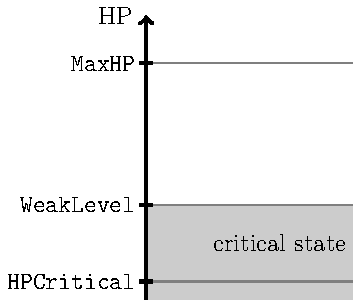
\includegraphics[width=0.3\linewidth]{002_simulation_structure/images/health_global.pdf}
    \caption{The health of the agents is represented by a HP value between \lstinline$HPCritical$ and \lstinline$MaxHP$. All HP values which are below \lstinline$WeakLevel$ are classed as critical. The diagram is not drawn to scale.}
    \label{fig:health_system}
\end{figure}

\subsection{Food and Health: \lstinline$updateHP$}\label{updateHP}
To increase their HP, agents need to eat. However, the amount an agent's HP improves can saturate in a single day; eating more than a certain amount will provide an agent with no extra benefit to their HP. Moreover, eating more food will lead to diminishing returns in terms of HP change. Mathematically, the ideas of diminishing returns and saturation are well captured by the step response of a 1st-order system:

\begin{equation}\label{updateHP_general}
   \text{newHP}= \text{currentHP} +\underbrace{w(1-e^{\frac{-\text{foodTaken}}{\tau}})}_{\text{HPChange}}
\end{equation}

where the two parameters $w$ and $\tau$ are defined at the beginning of the simulation. The shape of this curve is given in \Cref{fig:updateHP} together with some important parameters.

\begin{figure}[htb]%
    \centering
    \subfloat[\centering Overview]{{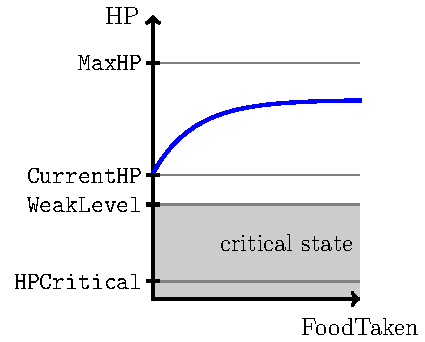
\includegraphics[width=0.36\linewidth]{002_simulation_structure/images/health_updateHP_overview.pdf}}}%
    \qquad
    \subfloat[\centering Detailed representation]{{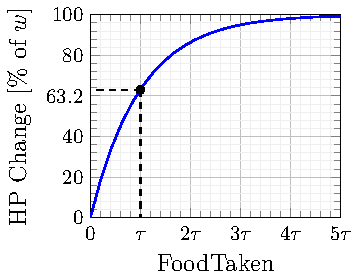
\includegraphics[width=0.36\linewidth]{002_simulation_structure/images/health_updateHP_detailed.pdf}}}%
    \caption{\texttt{updateHP} as a function of the amount of food eaten (``FoodTaken'').}%
    \label{fig:updateHP}%
\end{figure}

It is not possible to gain more HP than $w$ over the duration of one day; this is an intentional limit to prevent an agent's health from improving too quickly. As an example, we can think of an agent that starts from the weak level and wants to reach the maximum HP value. It would take several days for this agent to ``recover'' from this weak level and stabilise its health to a high HP value. 

Note that it is possible for an agent to achieve an HP value that is larger than \texttt{MaxHP} inside \lstinline$hpDecay()$. At the end of each day, the \lstinline$hpDecay()$ function will apply the cost of living and then bound the final HP value by \lstinline$MaxHP$.


As a special case, an agent reaching the critical state will be treated differently. For these agents, the HP update rule is the following:

\begin{equation}\label{updateHP_critical}
    \text{newHP} = \min\left\{\text{HPCritical}+\text{HPReqCToW}, \text{currentHP} +w\cdot(1-e^{-\text{foodTaken}/ \tau})\right\}
\end{equation}

%
%%%%%%%% Costs of Living: hpDecay
%
\subsection{Costs of Living: \texttt{hpDecay}}\label{hpDecay}
At the end of each day, the HP value of the agents will be reduced by the cost of living. The cost of living is larger for an agent with larger HP value than for an agent with lower HP value. This fact is motivated by a simple observation: humans that have stronger bodies and immune systems also need more food to sustain their level of health. The exact relation between HP value, cost of living, and HP value after applying the cost of living is given by the following linear relation:

\begin{equation}\label{hpDecay}
    \text{newHP} = \text{currentHP}-\left[b + (\text{currentHP-WeakLevel})\cdot s\right]
\end{equation}


where $b$ is a (constant) base cost, and $s$ is the slope of the linear function. These parameters are initialized at the beginning of the simulation. \ToDo{Add a diagram for this?}

To ensure that the HP value at the end of the day is bounded by \texttt{maxHP}, we slightly modify the above expression:

\begin{equation}\label{hpDecay_bounded}
    \text{newHP} =\max\left\{\text{MaxHP}, \text{currentHP}-\left[b + (\text{currentHP-WeakLevel})\cdot s\right]\right\}
\end{equation}

Once again, the agents in the critical state are treated differently. If, by the end of the day, they achieved to gain \texttt{HPReqCToW} HP, meaning if their HP after eating is

\begin{equation}\label{HPReqCToW}
    \text{currentHP} \geq \text{HPCritical}+\text{HPReqCToW},
\end{equation}

they will be upgraded to the \texttt{WeakLevel}:

\begin{equation}\label{hpDecay_critical_upgrade}
    \text{newHP} = \text{WeakLevel}
\end{equation}

On the other hand, if they do not fulfill the above condition, They will be kept in the critical state by setting their HP to

\begin{equation}\label{hpDecay_critical_stay}
    \text{newHP} = \text{HPCritical}
\end{equation}

and a counter named \texttt{daysAtCritical} will be increased by one. If \texttt{daysAtCritical} reaches \texttt{MaxDayCritical}, the agents die and are replaced. Note that the counter is reset to 0 if the agent exit the critical state.